\documentclass[12pt,a4paper]{article}
\usepackage[brazil]{babel}
\usepackage[utf8]{inputenc}
\usepackage[tmargin=2cm, bmargin=2cm, lmargin=2cm, rmargin=2cm]{geometry}
\usepackage{graphicx}
\usepackage{float}
\usepackage{indentfirst}
\usepackage[pdftex]{hyperref}
\usepackage{enumerate}
\usepackage{amsthm,amssymb,amstext,amsmath}
\usepackage{verbatim}
\usepackage{amsmath}
\usepackage{eucal}
\usepackage{mathrsfs}
\usepackage[utf8]{inputenc}
\usepackage{hyperref}
\usepackage{fancyvrb}
\DefineVerbatimEnvironment{code}{Verbatim}{fontsize=\small}
\DefineVerbatimEnvironment{example}{Verbatim}{fontsize=\small}

\title{Projeto Final\\MAC0426 - Sistemas de Bancos de Dados}
\author{
    André Meneghelli Vale - 4898948\\
    \texttt{andredalton@gmail.com}
}
\date{}

\pdfinfo{%
  /Title    ()
  /Author   ()
  /Creator  ()
  /Producer ()
  /Subject  ()
  /Keywords ()
}

\begin{document}
\clearpage\maketitle
\thispagestyle{empty}



\newpage

\section{Descrição do domínio de dados.}

\subsection{Dados necessários ao sistema.}

O sistema cujo banco de dados foi desenvolvido tem o objetivo de gerenciar informações sobre imagens de projetos e produtos que interessam a profissionais da área de arquitetura e afins. Este projeto consiste em uma relação de imagens de projetos que utilizam determinados produtos em sua composição. Por exemplo as telhas de uma casa ou os móveis expostos à chuva.

Os usuários possíveis para esta aplicação são:

\begin{itemize}
\item \emph{Arquitetos}: Unicos usuários que podem cadastrar projetos e produtos. Para tanto é necessária a validação do CREA deste usuário.
\item \emph{Administrador}: Usuários responsáveis pela liberação de acesso dos arquitetos à aplicação. São os únicos capazes de visualizar os logs de modificação do sistema.
\item \emph{Usuário comum}: Pessoas que têm interesse em comentar algum projeto ou produto (Os comentários não podem ser anônimos).
\end{itemize}

As senhas de acesso são salvas já codificadas usando o algoritmo MD5, sendo que antes de serem codificadas ainda recebem um prefixo gerado aleatóriamente para cada um dos usuários. Esta medida tem o objetivo de aumentar a segurança no armazenamento das senhas de cada um dos usuários, dificultando assim o uso de tecnicas de desemcriptação mesmo para quem tem acesso ao banco de dados.

As imagens serão salvas em diretório e o banco de dados é responsável pelo armazemamento das informações textuais das descrições do projeto, contas de acesso ao sistema, registros de alteração nos dados e comentários dos usuários.

\newpage

O domínio dos dados necessários serão, em sua grande maioria, campos textuais:

\begin{itemize}
\item \emph{VARCHAR}
\subitem \emph{cidade}: nome (255);
\subitem \emph{estado}: nome (255);
\subitem \emph{fabricante}: nome (255), homepage (255), email (255);
\subitem \emph{fornecedor}: nome (255), homepage (255), email (255), rua(255), cep (10);
\subitem \emph{produto}: nome (255);
\subitem \emph{produto\_acesso}: url\_origem (255);
\subitem \emph{projeto}: titulo (255);
\subitem \emph{projeto\_acesso}: url\_origem (255);
\subitem \emph{registro}: descricao (255);
\subitem \emph{usuario}: nome (255), homepage (255), email (255), CREA (255).
\item \emph{TEXT}
\subitem \emph{pruduto\_comentario}: comentario;
\subitem \emph{projeto\_comentario}: comentario;
\subitem \emph{pruduto}: descricao;
\subitem \emph{projeto}: descricao.
\item \emph{CHAR}
\subitem \emph{usuario}: senha (32), semente (3);
\subitem \emph{estado}: sigla (2).
\item \emph{DATETIME}
\subitem \emph{registro}: data;
\subitem \emph{projeto\_comentario}: data;
\subitem \emph{produto\_comentario}: data;
\subitem \emph{projeto\_acesso}: data;
\subitem \emph{produto\_acesso}: data.
\item \emph{ENUM}
\subitem \emph{usuario}: tipo (arquiteto, comum, administrador).
\item \emph{INT}: todos os identificadores de tabelas são do tipo inteiro, assim como as suas respectivas chaves estrangeiras. Apenas o campo a seguir é do tipo \verb+INT+
\subitem \emph{fornecedor}: numero (10).
\end{itemize}

\subsection{Responsabilidades da aplicação.}

É de responsabilidade da aplicação fazer com que as imagens sejam salvas corretamente em diretórios assim como garantir acesso a elas através do identificador do projeto ou produto a que esta se refere. Na ultima sessão deste documento constam alguns exemplos de requisições possíveis de serem usadas neste projeto.


\section{Modelo lógico e conceitual.}
\begin{figure}[ht!]
\centering
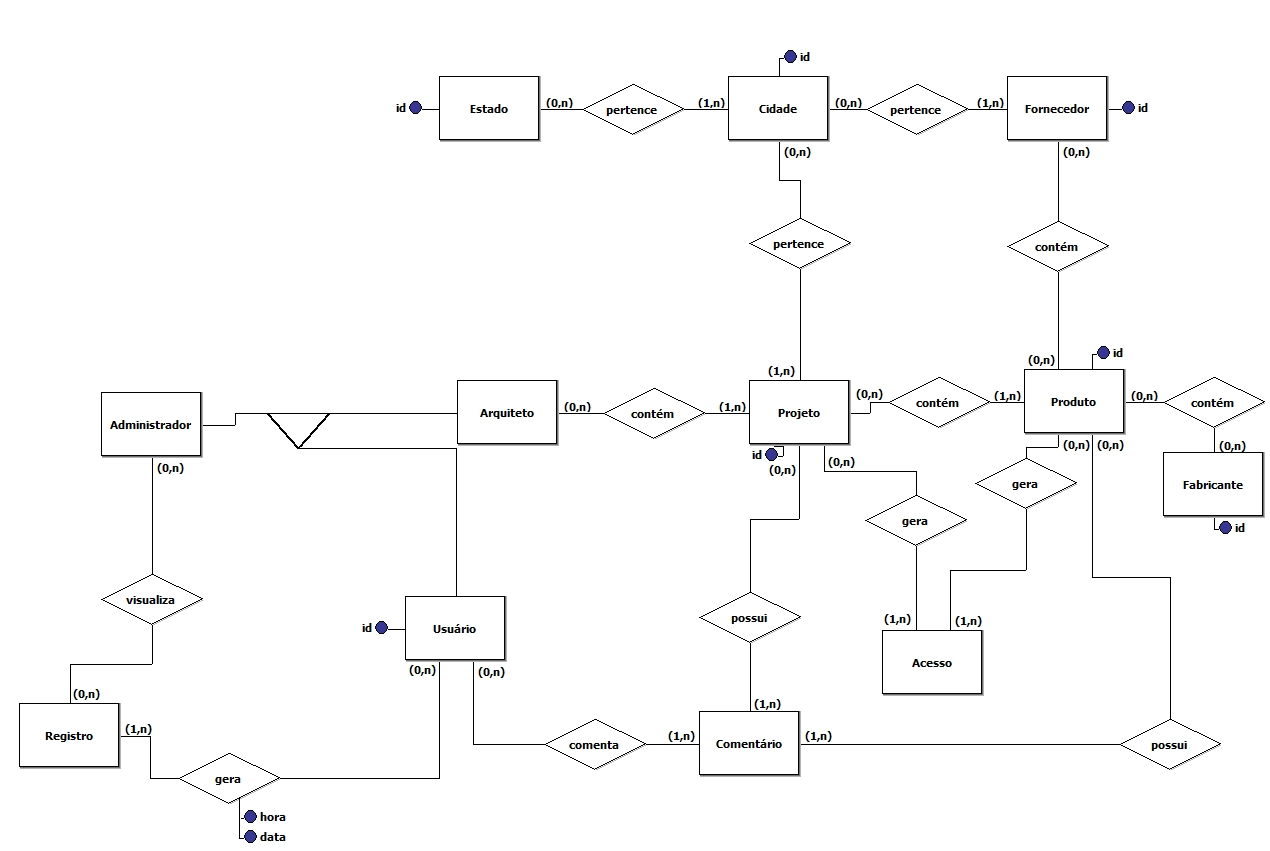
\includegraphics[width=180mm]{BD_conceitual.jpg}
\caption{Modelo Conceitual}
\label{overflow}
\end{figure}

\newpage

\begin{figure}[ht!]
\centering
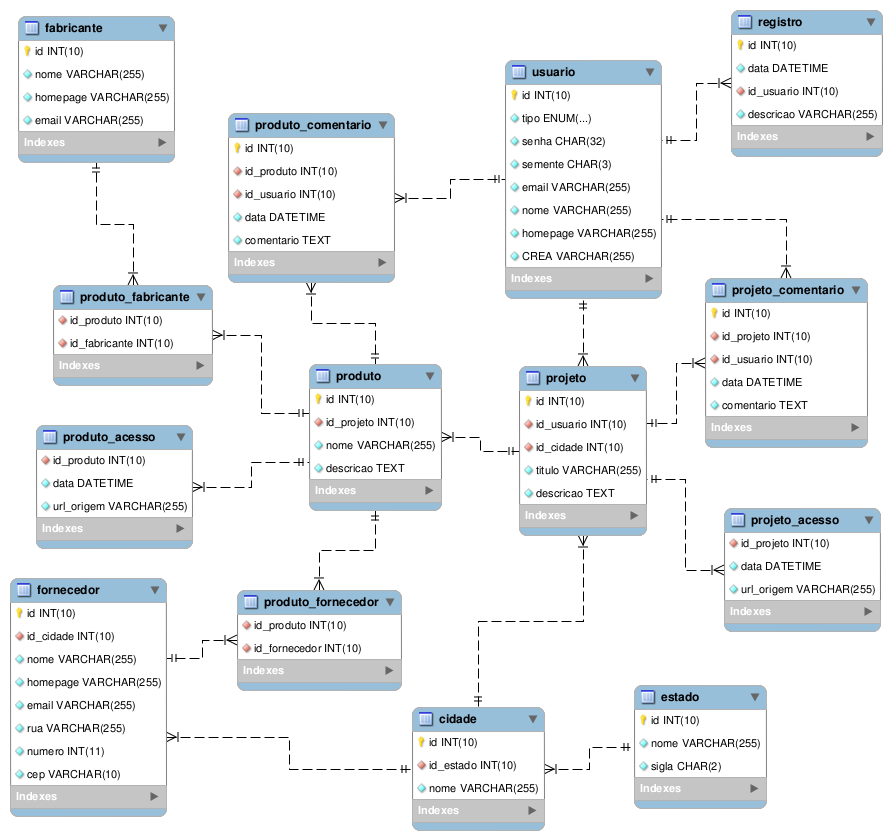
\includegraphics[width=180mm]{Modelo_fisico.png}
\caption{Modelo Lógico}
\label{overflow}
\end{figure}

\newpage

\section{Banco de dados em MySQL.}

O banco de dados foi desenvolvido em MySQL e contém apenas exemplos de dados a serem inseridos. Obviamente um sistema comercial de verdade deveria conter registros de modificação capaz de identificar a localização das respectivas ações. Assim como algum tipo de melhoria que permita que usuários sejam criados ou recuperem senhas a partir dos emails cadastrados.

Parte das informações foram colhidas de fontes na internet. Principalmente \href{http://wikipedia.org/}{wikipedia} para as informações sobre municípios e descrições relevantes sobre as obras de Oscar Niemeyer. Todos os comentários foram gerados a partir do \href{http://www.lerolero.com/}{Gerador de LeroLero}.
\\
\\
Segue o arquivo \verb+SQL+ do banco de dados: \url{projetoBD.sql}

\section{Consultas significativas.}

\begin{itemize}
\item Tenta acessar os dados do \verb+usuário+ com \verb+email ucomum@hotmail.com+ e \verb+senha comum+ (caso a aplicação transmita a senha sem encriptação):
\begin{code}
SELECT * FROM usuario
WHERE
    MD5(CONCAT(semente, 'comum')) = senha
    AND email = 'ucomum@hotmail.com';
\end{code}

\item Tenta acessar os dados do usuário com email \verb+andredalton@gmail.com+ com a \verb+senha+ e a \verb+semente+ encriptadas no lado do cliente:
\begin{code}
SELECT * FROM usuario
WHERE
    'd5f91c925cd3191f2b3187bd1da00036' = senha
    AND email = 'ucomum@hotmail.com';
\end{code}

\item Seleciona todos os \verb+estados+ cadastrados no banco de dados:
\begin{code}
SELECT * FROM `estado`;
\end{code}

\item Seleciona todas as \verb+cidades+ do \verb+estado+ \emph{SP}:
\begin{code}
SELECT * FROM `cidade`
WHERE id_estado = (SELECT * FROM `estado` WHERE sigla = 'SP');
\end{code}

\item Insere um novo \verb+projeto+ do \verb+usuário+ de id \verb+3+ na cidade de \verb+Apiaí(23)+:
\begin{code}
INSERT INTO `projeto`(`id_usuario`, `id_cidade`, `titulo`, `descricao`)
VALUES
    (3, 23, 'Casa Rural - Rustic Wild', 'Uma casa rural para o bom caboclo.');
\end{code}

\item Altera o \verb+fornecedor 1+ para \verb+2+ em todos os seus \verb+produtos+:
\begin{code}
UPDATE `produto_fornecedor`
SET `id_fornecedor`=2 WHERE `id_fornecedor`=1
\end{code}

\item Remove os \verb+registros+ anteriores ao ano de \verb+2013+:
\begin{code}
DELETE FROM `registro` WHERE data < "2013";
\end{code}

\newpage
\item Modifica todos os \verb+fornecedores+ dos \verb+produtos+ fabricados pelo \verb+fabricante 3+ para o \verb+fornecedor 1+:
\begin{code}
UPDATE `produto_fornecedor`
SET `id_fornecedor`=1
WHERE
    `id_produto` IN
    (
        SELECT `id_produto` FROM `produto_fabricante`
        WHERE `id_fabricante` = 3
    )
\end{code}

\item Conta quantos comentários os \verb+produtos+ fabricados pelo \verb+fabricante 4+ e fornecidos pelo \verb+fornecedor 3+ receberam:
\begin{code}
SELECT
    COUNT(*) as total
FROM
    produto_comentario pc
    INNER JOIN produto_fabricante pf ON pf.id_produto = pc.id_produto
    INNER JOIN produto_fornecedor pfo ON pfo.id_produto = pc.id_produto
WHERE
    pf.id_fabricante = 4
    AND pfo.id_fornecedor = 3;
\end{code}

\item Seleciona o \verb+titulo+ do \verb+projeto+ mais comentado do \verb+usuário 3+:
\begin{code}
SELECT p.titulo
FROM projeto p
WHERE p.id_usuario = 3
GROUP BY id
ORDER BY COUNT(*)
LIMIT 1;
\end{code}

\item Seleciona os \verb+10 comentários+ mais recentes dos \verb+produtos+ da ultima semana:
\begin{code}
SELECT * FROM produto_comentario
WHERE data > DATE_SUB(NOW(),INTERVAL 1 WEEK)
ORDER BY data DESC
LIMIT 10;
\end{code}

\end{itemize}

\newpage
\begin{thebibliography}{99}
\bibitem{Obras de Oscar Niemeyer}
\url{http://pt.wikipedia.org/wiki/Anexo:Lista_de_obras_de_Oscar_Niemeyer}
\bibitem{SQL}
\url{http://www.w3schools.com/sql/}
\bibitem{LaTeX}
\url{http://www.maths.tcd.ie/~dwilkins/LaTeXPrimer/}
\end{thebibliography}
\thispagestyle{empty}
\end{document}